\documentclass{article}

% New commands declaration

\usepackage[frenchb]{babel}
\usepackage[T1]{fontenc}

\usepackage{natbib,bibentry}
\usepackage{color}

\usepackage{yfonts}
\usepackage{graphicx}
\usepackage{epsfig,subfigure}
\usepackage{amsmath,amssymb,amsfonts}
\usepackage{calc}
\usepackage{float}
\usepackage{import}


\DeclareGraphicsExtensions{.eps, .jpg, .png}

\parindent = 0mm

\bibliographystyle{plain}

\hoffset = -20mm
\voffset = -25mm
\textwidth = 160mm
\textheight = 240mm

\definecolor{lightgray}{gray}{0.2}

\newcommand{\expect}{{\rm I \mkern-2.5mu \nonscript\mkern-.5mu E}}
\newcommand{\equaldef}{\stackrel{d}{=}}
\newcommand{\argmax}{\operatornamewithlimits{argmax}}

\newcommand{\debutrep}[1]{\color{blue}\begin{center} \hrulefill \textbf{ #1 } \hrulefill \end{center} }
\newcommand{\finrep}{\vspace*{5mm}\hfill $\square$\color{black}\vspace*{5mm}}

\begin{document}

\baselineskip = 4mm
\title{Traitement des Signaux Aléatoires: \\
Prédiction linéaire d'un signal par modélisation Auto-Régressive \\
Application au débruitage}

\author{\textbf{4 ETI -- CPE Lyon }\\[3mm]
{Travaux Pratiques TSA}}
\date{2020-2021}

\maketitle

\noindent\fbox{
\parbox{\linewidth-2\fboxrule-2\fboxsep}
{ 
\vspace*{2mm}
{\large\bf Noms, Prénoms: Philippe CHARRAT - Axel BRUYERE}\\[3mm]
{\large\bf Groupe: D - Binôme 2}\\[3mm]
{\large\bf Date: 04/11/20}\\[2mm]}}
\vspace*{5mm}



{\Large\bf Objectif}~--~~\begin{minipage}[t]{135mm}
Débruitage d'un enregistrement sonore par prédiction linéaire basée sur un modèle auto-régressif.

\vspace*{4mm}
L'ensemble des fonctions Matlab nécessaires est à récupérer sur la  plateforme {\em CPe-campus} sous l'archive {\tt Fichiers\_TP\_AR.zip}.
\end{minipage}

\vspace*{4mm}
\renewcommand{\thesection}{\Roman{section}}

\section{Préparation : Modélisation auto-régressive d'un signal aléatoire}

Soient $(s_n,\,n=1,\ldots, N)$, les échantillons d'un signal aléatoire réel, stationnaire. On se propose de trouver \textbf{un modèle} tel que l'on puisse prédire linéairement la valeur de $s_n$  à partir des échantillons précédents de $s$
\begin{equation}
\hat{s}_n = \sum_{k=1}^{\infty} h[k]\,s_{n-k}.
\label{eq:AR(M)}\end{equation}
Il s'agit donc de déterminer les coefficients  $h[k]$, $k=1,2,\ldots$  minimisant l'erreur de prédiction:
\begin{equation}
\varepsilon_n = s_n - \hat{s}_n = s_n - \sum_{k=1}^{\infty} h[k] s_{n-k}
\label{eq:erreur}
\end{equation}
au sens de l'erreur quadratique  moyenne (i.e. puissance moyenne minimale) $P_{\varepsilon} = \mathbb{E}\{ \varepsilon^2_n\} = \sigma^2$

\subsection{}
Quel principe de construction  permet de garantir une erreur quadratique moyenne minimale? \\

\debutrep{réponse}

\finrep

\subsection{}
Par application de ce principe, montrer que l'erreur de prédiction $\varepsilon_n$ est  un bruit blanc.\\

\debutrep{réponse}

\finrep

\subsection{}
\label{eq.3} 
En pratique, il faut limiter  l'ordre du modèle à $M<\infty$. Dans ces conditions et toujours par application de ce même principe de construction, établir le système d'équations linéaires, dont les coefficients $\{h[k],~k=1,\ldots M\}$ sont les solutions.\\

\debutrep{réponse}

\finrep


\subsection{}
Calculer la puissance de l'erreur de prédiction $P_{\varepsilon}$ en fonction de l'autocorrélation $\gamma_s(k)$ du signal et des coefficients $\{h[k],~k=1,\ldots M\}$.\\


\debutrep{réponse}

\finrep

\subsection{}
\label{eq.5}
Insérer cette relation dans le système 	d'équations linéaires  obtenu à la question \ref{eq.3}.\\

\debutrep{réponse}

\finrep


\clearpage
\section{Manipulation}

\subsection{Signal et contexte}
Charger le signal audio {\tt ProtestMonoBruit.wav} avec la commande:\\[1mm]
{\tt
[s,Fs]= audioread('ProtestMonoBruit.wav') ;\\[1mm]
}
où $s$ et $Fs$ correspondent respectivement au signal échantillonné et à la fréquence d'échantillonnage.

En indiquant le code correspondant, afficher le signal (axe temporel gradué en secondes). Les pics aléatoires superposés au signal sont une affection classique des sons numérisés à partir de disques vinyles, qui se manifestent par un  \textit{bruit de craquement} lorsqu'on écoute le fichier audio:\\[1mm]
{\tt
sound(s,Fs) ;\\[2mm]
}
\begin{figure}[!h] 	
    \centering
    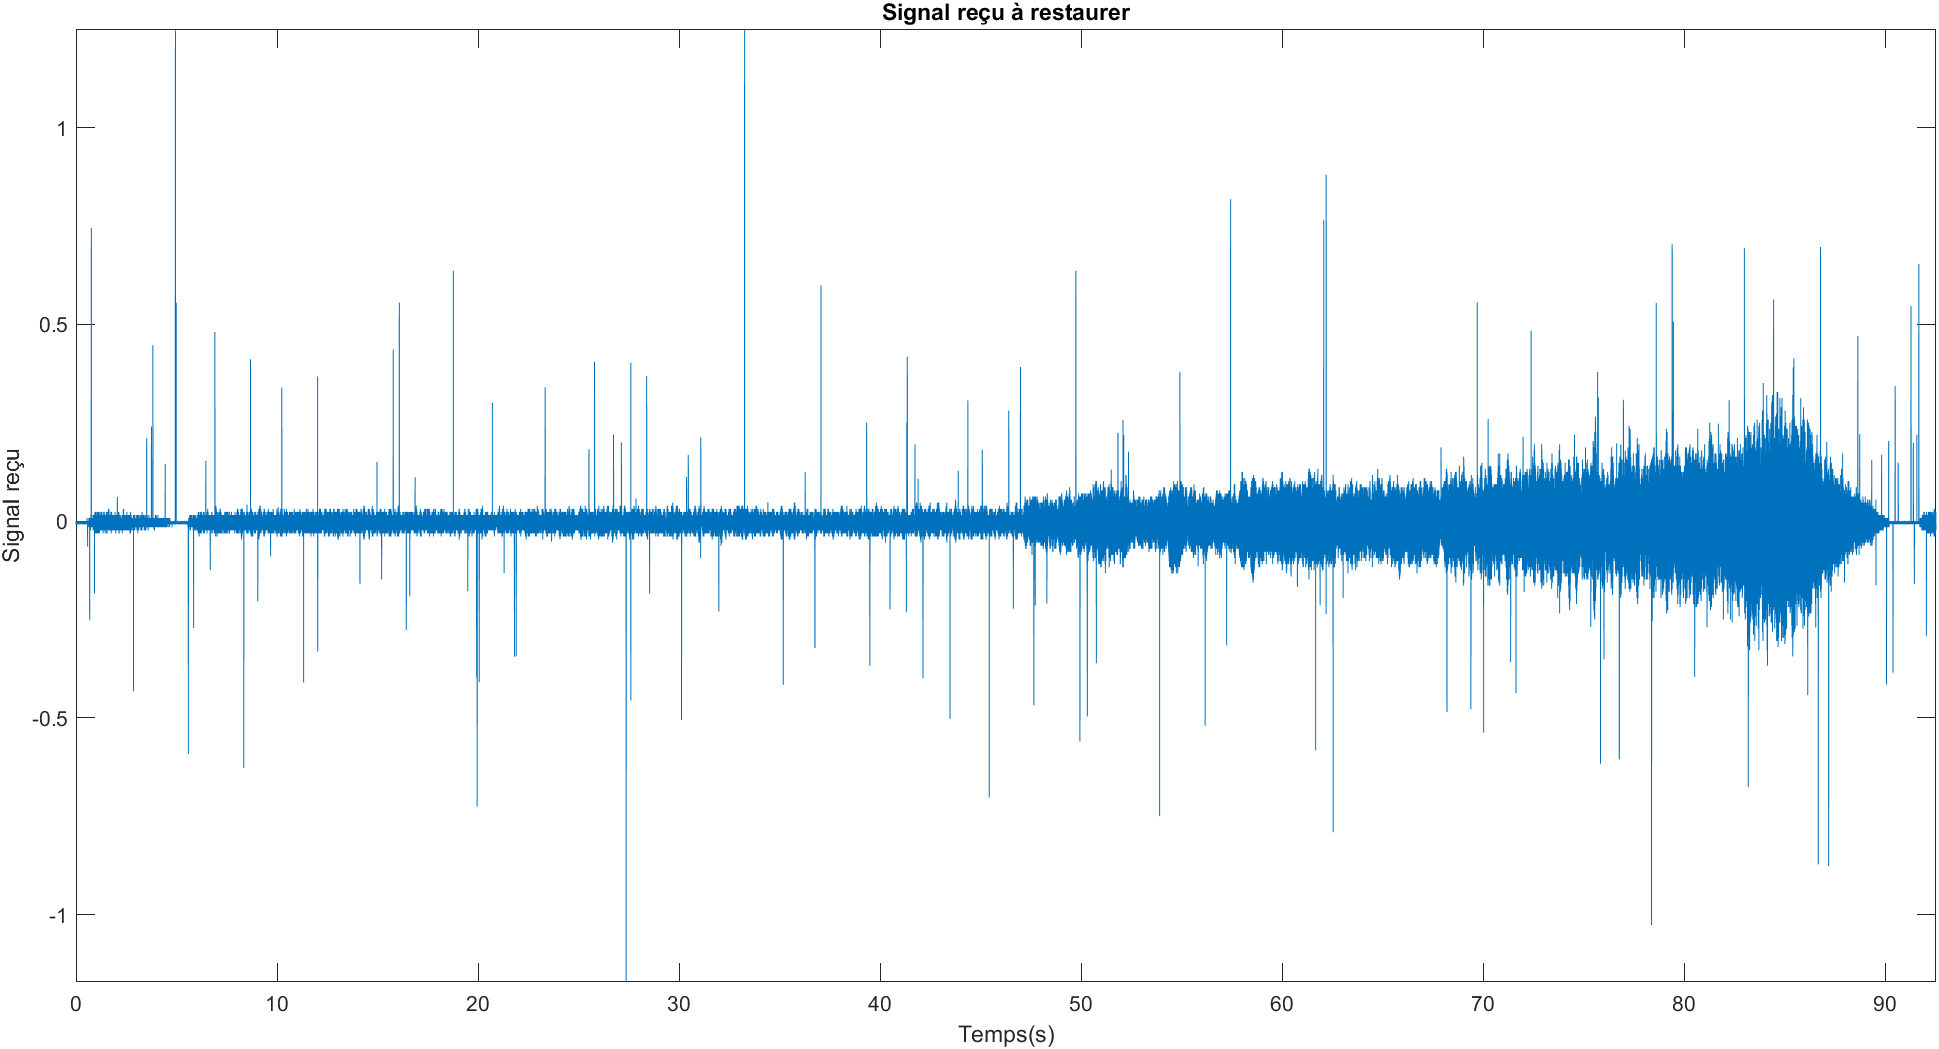
\includegraphics[width=1\textwidth]{images/signalorigine.png}
    \caption{Signal d'origine bruité}
    \label{fig-binaire}
\end{figure}

On se propose de restaurer le signal initial en {\em débruitant} l'enregistrement.\\
Quelle(s) solution(s) simple(s) pourrait on envisager pour supprimer (ou atténuer) l'effet de ces pics? En quoi ne seraient elles pas satisfaisantes ?\\ 
\\
Pour essayer de débruiter ce signal, l'une des méthodes "simple"  consisterait a définir un seuil. Ce palier correspondrait à  l'amplitude maximale de la musique, et nous pourrions ainsi filtrer les amplitudes supérieures (donc atténuer les parasites). Cette méthode pose deux problèmes : premièrement elle ne va pas débruiter mais seulement atténuer le bruit. Le second problème est que nous ne pourrions pas "facilement" imposer un seuil, car il faudrait pouvoir discerner le signal utile du bruit. \newline


\vspace*{3mm}
La solution retenue ici, consiste à modéliser l'enregistrement audio (qui n'est pas un bruit blanc!) par un \textbf{processus auto-régressif d'ordre M }($AR(M)$). Ce modèle est ensuite utilisé pour prédire l'échantillon  $s_n$ du signal à partir des $M$ échantillons précédents $\{s_{n-m},\,1 \leq m \leq M)\}$ . Puisque l'apparition des pics de craquement est \textbf{aléatoire} et supposée \textbf{indépendante} du signal, le modèle $AR(M)$ n'aura pas le pouvoir de  les prédire.

\newpage
\subsection{Estimation de la fonction d'autocorrélation.}

Pour limiter les temps de calcul, on limitera l'analyse du signal à l'intervalle $t\in[60,70]$ secondes. \\
Sur ce segment, estimer la fonction d'autocorrélation $\gamma_s[k] = \gamma_s(kTs)$, 
% (avec $\gamma_s(0)=1$), 
pour $-K\leq k \leq K$. Pour cela, on utilisera l'instruction suivante:  {\tt [R,lags] = xcorr(x,K,'biased')}, où $R$ est le vecteur des corrélations et {\tt lags}, le vecteur des retards $-K\leq k \leq K$. Afficher le code correspondant et le résultat pour $K=200$ (on n'hésitera pas à faire un zoom autour de la zone d'intérêt\ldots) \\ \\
Le code de cette partie est le suivant :  
\begin{verbatim}
    %Initialisation des variables
    K = 200
    indice_temps_60 = find(temps==60);
    indice_temps_70 = find(temps==70);
    
    % Création des vecteurs de temps et de données d'une durée de 10 secondes
    time2 = temps(indice_temps_60:indice_temps_70);
    s2 = s(indice_temps_60:indice_temps_70);
    
    % Calcul de l'autocorrélation à l'aide de la fonction xcorr (native à MATALB)
    [R,lags] = xcorr(s2,K,'biased');
    
    %Partie affichage (Tronquée pour la lisibilité du rapport) 
\end{verbatim}

Nous obtenons les figure suivante ; 
\begin{figure}[!h] 	
    \centering
    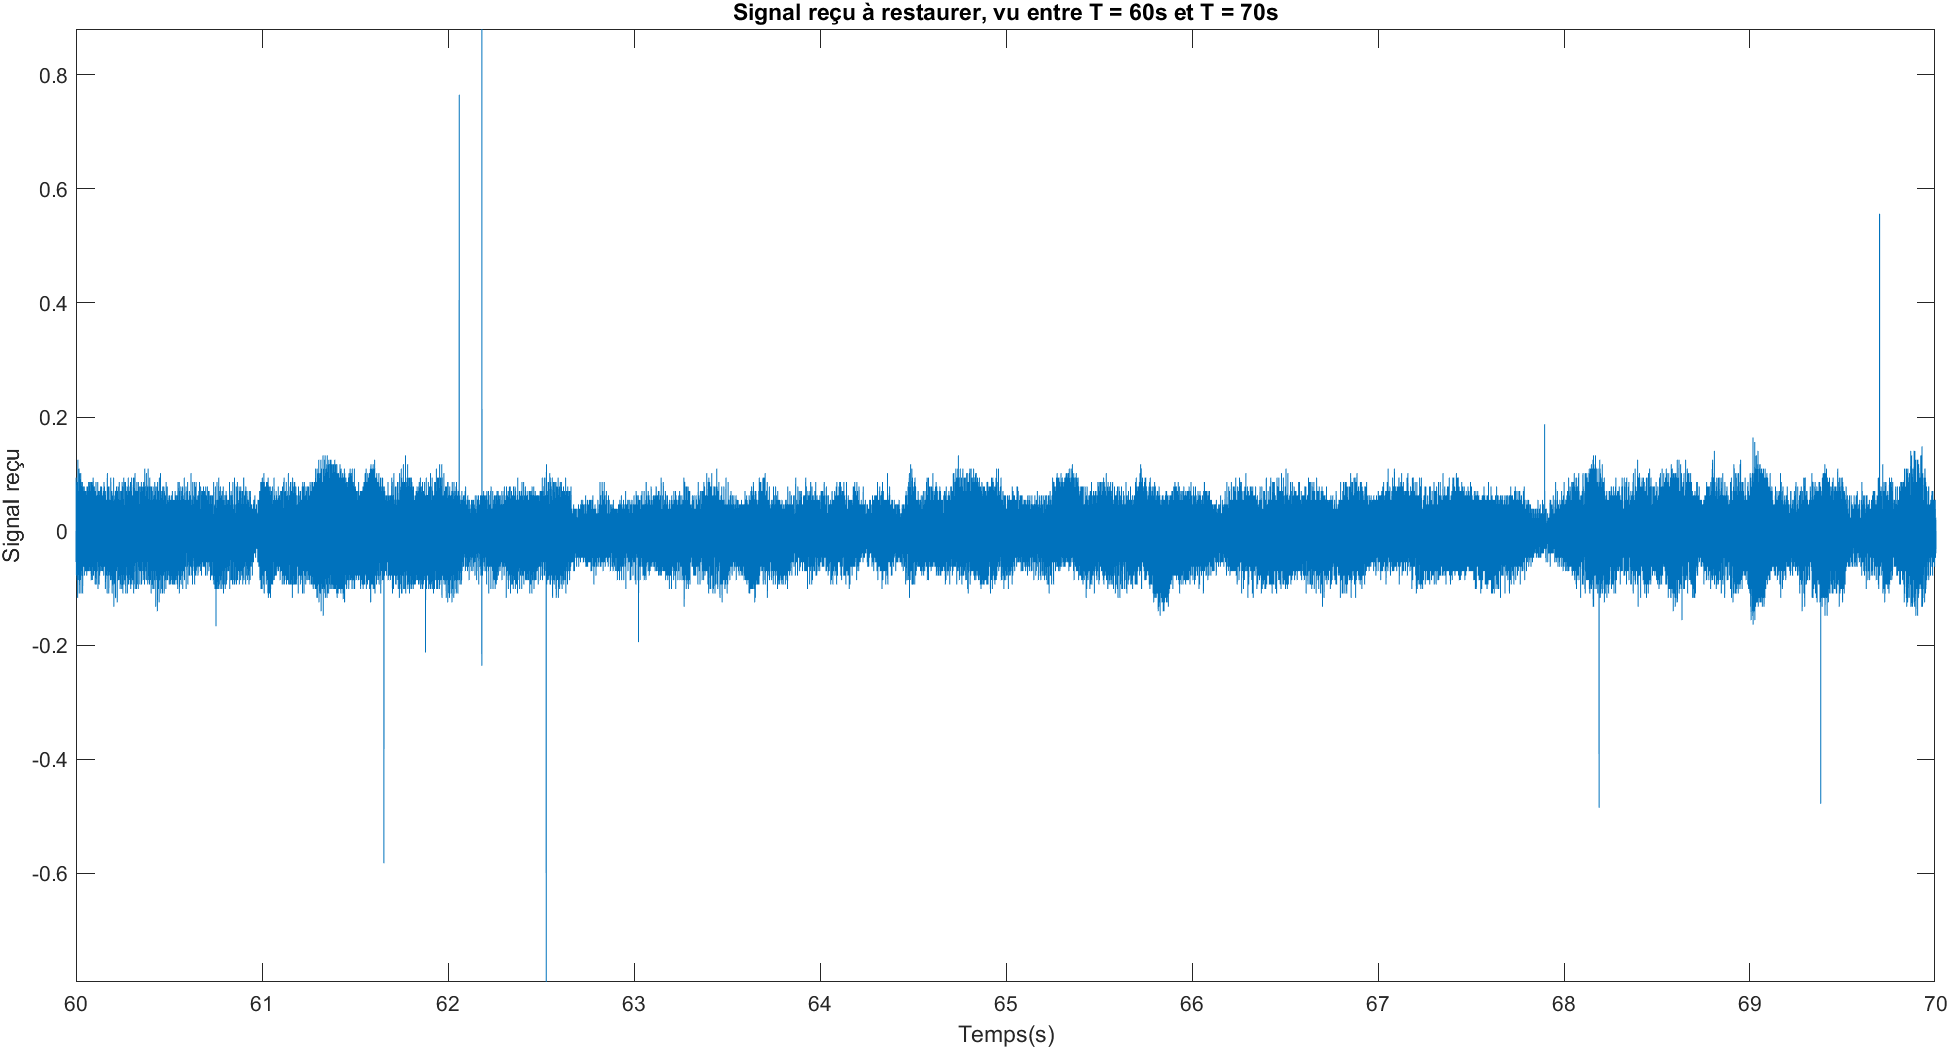
\includegraphics[width=1\textwidth]{images/signaloriginecourt.png}
    \caption{Section du Signal entre 60 et 70 secondes}
    \label{fig-binaire}
\end{figure}
nous pouvons observer que l'on obtient un signal qui dure 10 secondes, L'amplitude moyenne du signal est approximativement 0.015 (méthode graphique), et l'on observe une dizaine de pics qui peuvent être considérés comme parasites. \\

\clearpage
\begin{figure}[!h]
    \centering
    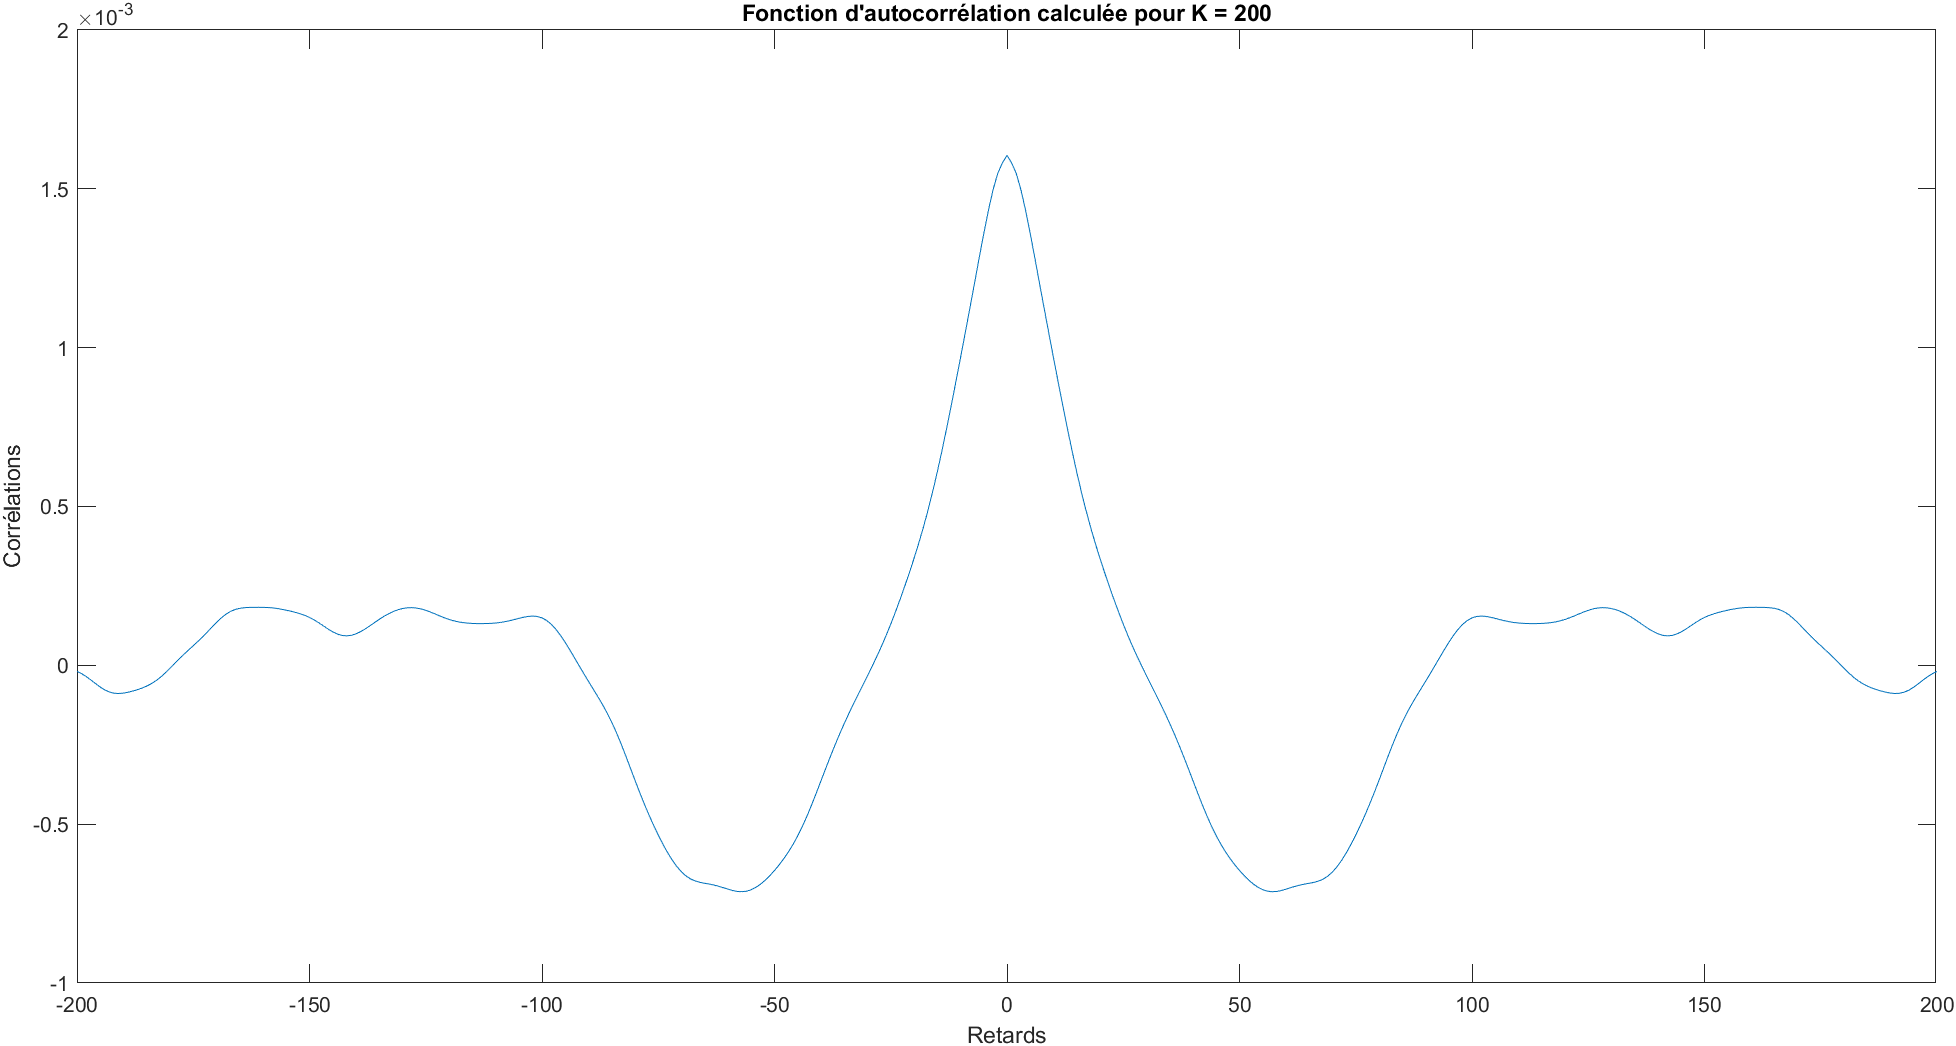
\includegraphics[width=1\textwidth]{images/convo.png}
    \caption{Fonction d'auto-corrélation du signal entre 60 et 70s}
    \label{fig-binaire}
\end{figure}
Nous pouvons observer sur la figure 3, la corrélation entre les échantillons. La fonction est symétrique en zéro, à l'aide des propriétés de symétrie Hermitienne nous pouvons en déduire que le signal est réel. \\
\newline
A partir de cette fonction, justifier le choix $M \approx 20$ pour l'ordre du modèle $AR(M)$.\\
\newline
Graphiquement le $\pm$20ième échantillons correspond au premier indice à avoir une amplitude nulle. Ainsi, nous pouvons considérer que l'on en possède un nombre suffisant pour pouvoir récréer le signal. \\
Il est à noter que plus le nombre d'échantillons est important et meilleure est la précision d'estimation. Nous aurions pu prendre plus d'échantillons mais cela aurait augmenté significativement le temps de calcul, car certaines opérations sont coûteuses (Exemple : une inversion de matrice à M éléments). \\
En conclusion M = 20 est un choix cohérent car nous possédons un nombre suffisant d'indices pour estimer le signal tout en conservant un temps de calcul raisonnable. 

\newpage
\subsection{Identification du modèle $AR(M)$}

En fixant alors l'ordre du modèle auto-régressif à $M=20$, programmer et résoudre l'équation matricielle (complète) obtenue à la question  \ref{eq.5} de la préparation. Utiliser pour cela, la fonction {\tt toeplitz.m} de Matlab. \\[1mm]
\textbf{Note:} $\gamma_s$ est la fonction d'autocorrélation  \textbf{empirique} estimée à partir des échantillons de $s$. La matrice de Toeplitz de la question \ref{eq.5} de la préparation peut donc ne pas être inversible. On utilisera alors la commande {\tt pinv.m} de Matlab pour calculer la matrice pseudo-inverse (de Moore-Penrose) qui elle, existe toujours.\\[1mm]
Reproduisez ci-dessous, le code développé pour le calcul des coefficients.
 
\begin{verbatim}
    % Les variables R et lags sont issues de la fonction de xcorr
    % Initialisation des variables
    M = 20; % Valeur déterminée dans la partie 2.3
    lag_0 = find(lags==0);
    
    %Création du vecteur r pour la fonction toeplitz.m
    r = zeros(1,M+1);
    r(1) = R(lag_0);
    for k = 1:1:M
        r(k+1) = R(lag_0 + k);
    end
    
    %Création de la matrice de Toeplitz
    tpz = toeplitz(r);
    
    %Pseudo-inversion pour résoudre le système 
    inv_tpz = pinv(tpz);
    
    %Vecteur contenant les résultats du système
    result = zeros(M+1,1);
    result(1) = 1;
    
    %Matrice des h/sigma^2
    phi = inv_tpz*result;
    h = zeros(M+1,1);
    
    %Division des termes par phi(1) = 1/sigma^2
    for k = 1:1:M+1
        h(k) = -phi(k)/phi(1);
    end
    
    %On tronque le vecteur de son premier terme
    h = h(2:end);    
    
    %Partie affichage tronquée
\end{verbatim}

\clearpage
Afficher les coefficients  du modèle $AR(M)$ $\{h[k],~k=1,\ldots M\}$ ainsi obtenus.

\begin{figure}[!h]
    \centering
    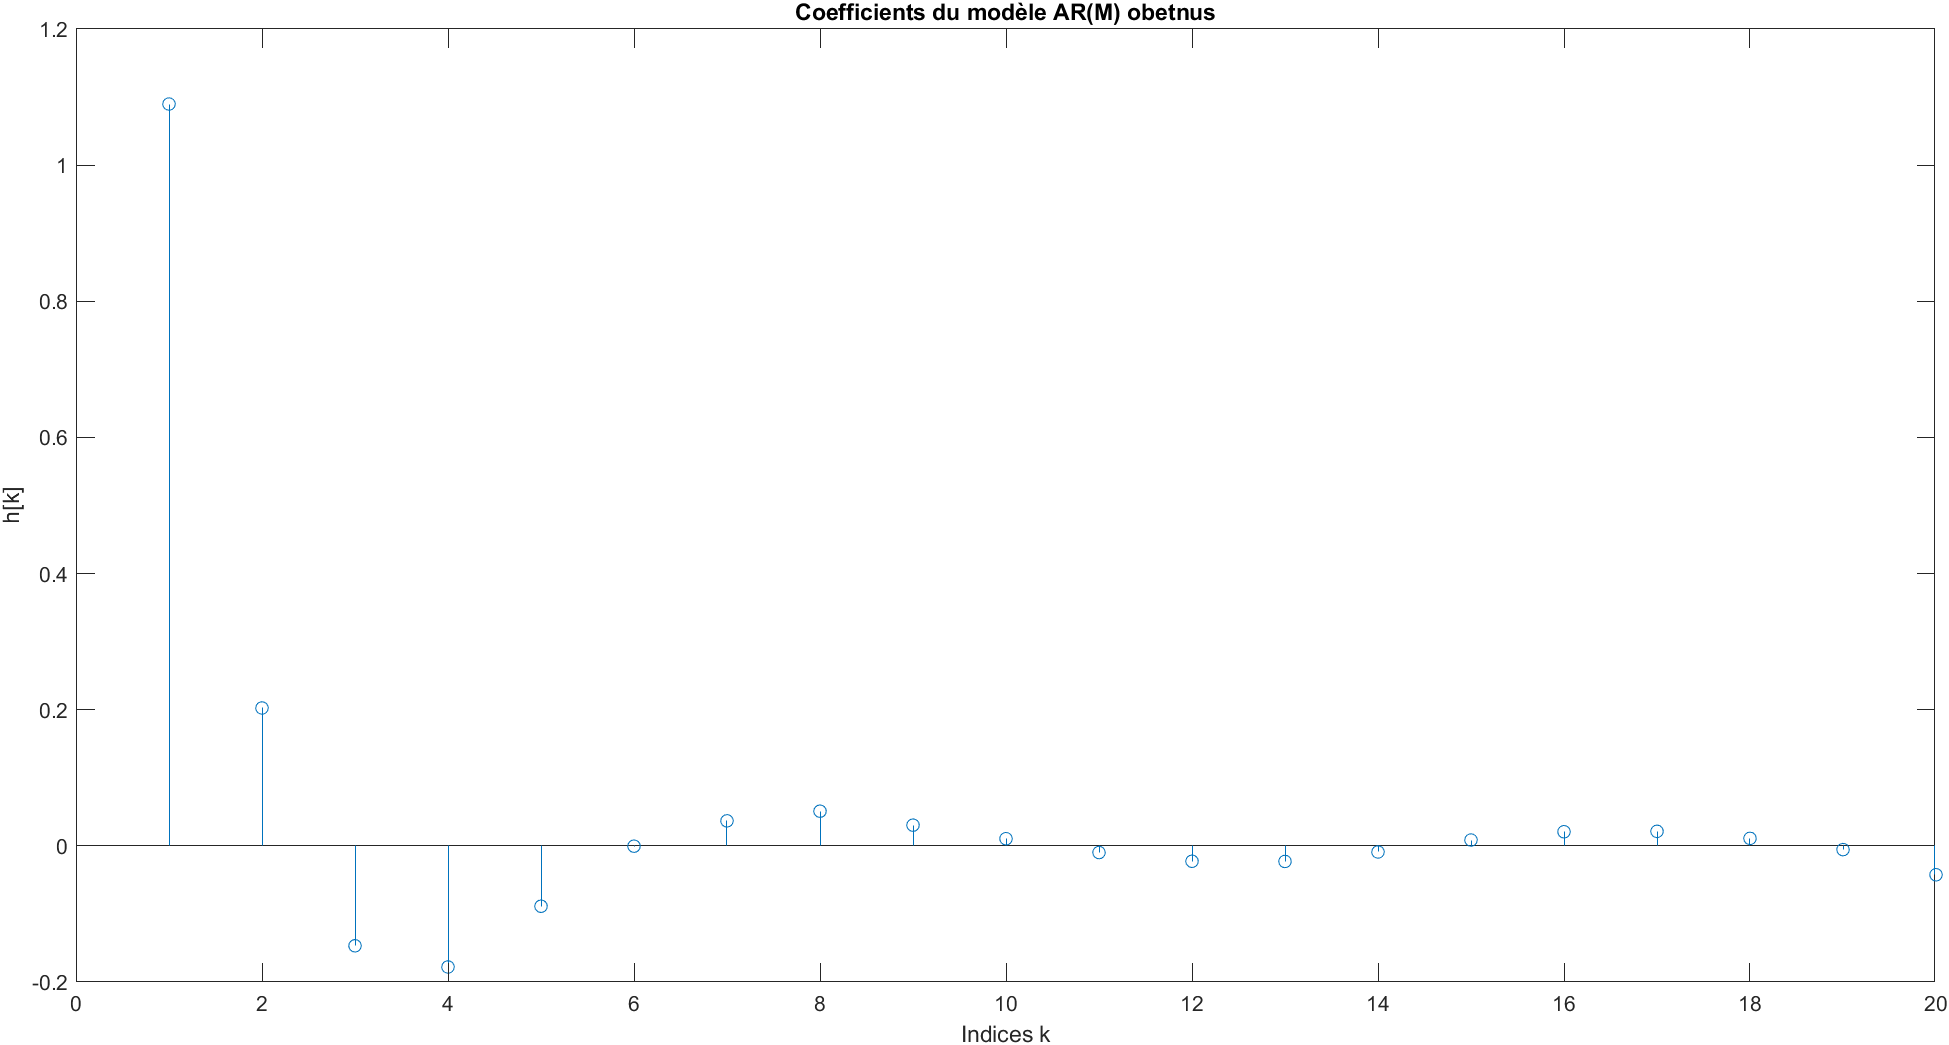
\includegraphics[width=1\textwidth]{images/hk_solution.png}
    \caption{Coefficients solutions du système d'équations linéaires h[k]}
    \label{fig-binaire}
\end{figure}
Pour obtenir ces coefficients, nous avons généré une matrice de Toeplitz à l'aide de la fonction \textit{toeplitz}. Nous l'avons ensuite inversée et multipliée par le vecteur de h[k]. Pour finir, nous avons posé un changement de variable pour obtenir le premier terme à 1 : nous avons multiplié tous les éléments du vecteur par l'inverse du premier terms.
\clearpage

\subsection{Prédiction linéaire}
\label{sec:predlin}

En utilisant les coefficients $(h[k],~k=1,\ldots,M)$ du modèle $AR(20)$ ainsi identifié, calculer la prédiction à un pas de temps $\hat{s}_n$ de $s_n$ à partir des échantillons précédents $(s_{n-k},~k=1,\ldots,M)$, pour $n \geq M+1$.\\[1mm]
Reproduisez ci-dessous, le code développé pour effectuer la prédiction et le calcul de l'erreur de prédiction.
\begin{verbatim}

    %Initialisation des variables
    p = 1;
    s_chapeau = zeros(1,length(s2));
    
    % Pour tous les éléments de la séquences supérieur à 20. 
    for n = indice_temps_60+20:indice_temps_70
        somme = 0;
        % Application de la formule : somme de 1 à M de h[k]*S(n-k)
        for k = 1:M
            somme = somme + h(k)*s(n-k);
        end
        % Ajout de la valeur dans le vecteur
        s_chapeau(p) = somme;
        p = p+1;
    end
    
    % Calcul de l'erreur quadratique moyenne
    erreur_quad = s_chapeau-s2';
    
    % Partie affichage
\end{verbatim}
 
Afficher (en {\tt subplot(211)}) la prédiction du signal ainsi obtenue superposée au  signal original et faites un zoom sur un craquement de votre choix.

Sur la même figure (en {\tt subplot(212)}) afficher la valeur absolue de l'erreur de prédiction $\varepsilon_n = \hat{s}_n - s_n$.

\begin{figure}[!h]
    \centering
    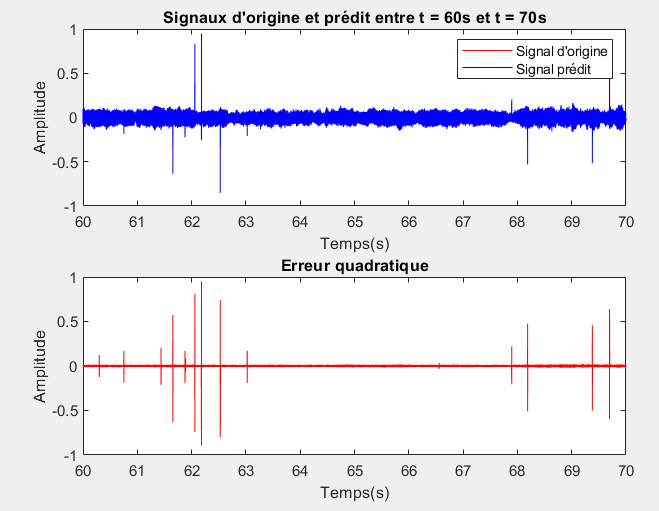
\includegraphics[width=1\textwidth]{images/global.png}
    \caption{Prédiction du signal, Signal Original et son erreur quadratique }
    \label{fig-binaire}
\end{figure}
\clearpage

\begin{figure}[!h]
    \centering
    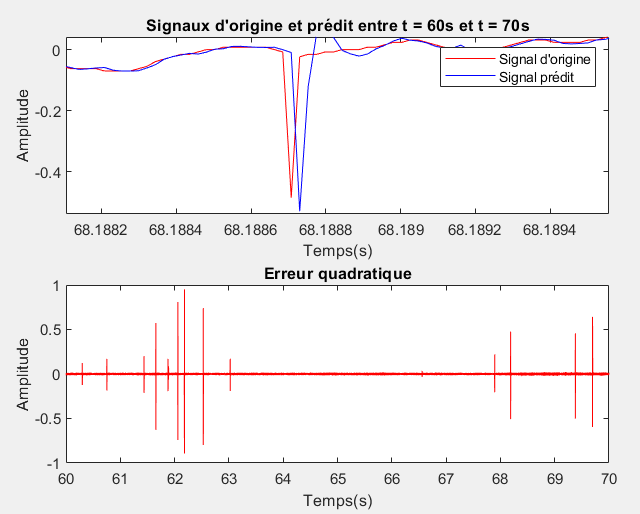
\includegraphics[width=1\textwidth]{images/zoom.png}
    \caption{Zoom sur l'un des craquements.}
    \label{fig-binaire}
\end{figure}

Nous constatons à l'aide de la figure 5 que les signaux sont très similaires. Si nous agrandissons l'intervalle (figure 6),  nous pouvons observer un décalage de l'ordre de quelques centièmes de seconde entre les deux signaux.\\ 
A noter que sur l'erreur quadratique, nous pouvons observer  de nombreux pics d'erreurs, en réalité un nombre supérieur au nombre de craquements. Ainsi, nous pouvons conclure que cette méthode est peu fiable car un certain nombre de "faux positifs" est décelé.\\
\clearpage

\subsection{Restauration par seuillage}

Choisissez un seuil $\Sigma$ pour identifier à partir de l'erreur de prédiction, les indices $k_i$ des dates de craquement.  Pour chacun de ces indices,  remplacer la valeur $s_{k_i}$ (i.e. craquement) par la valeur médiane (fonction {\tt median.m} sous Matlab) des échantillons de $s$ situés autour de $k_i$, $\{s_{k_i+l},~l=-10, -9,\ldots, 0 , \ldots 10\}$.

\begin{verbatim}
    % Initialisation du seuil à l'aide d'une méthode graphique
    seuil = 0.015;
    
    % Initialisation d'un vecteurs contenant tous les indices ou l'amplitude est supérieur au seuil
    crak = find(abs(erreur_quad)>=seuil);
    
    % Parcours du vecteur 
    for k = 1:1:length(crak)
        % La valeur du crak est remplacé par une valeur médian des 20 valeurs autours du craks.
        s_chapeau(crak(k)) = median(s(indice_temps_60+crak(k)-10:indice_temps_60+crak(k)+10));
    end
    
    % Calcul de la nouvelle erreur quadratique 
    erreur_quad = s_chapeau - s2';
    
    % Partie affichage 
\end{verbatim}

Afficher le signal ainsi restauré  superposé au signal original bruité (faire un zoom sur la même plage de signal qu'à la question \ref{sec:predlin}).\\

\begin{figure}[!h]
    \centering
    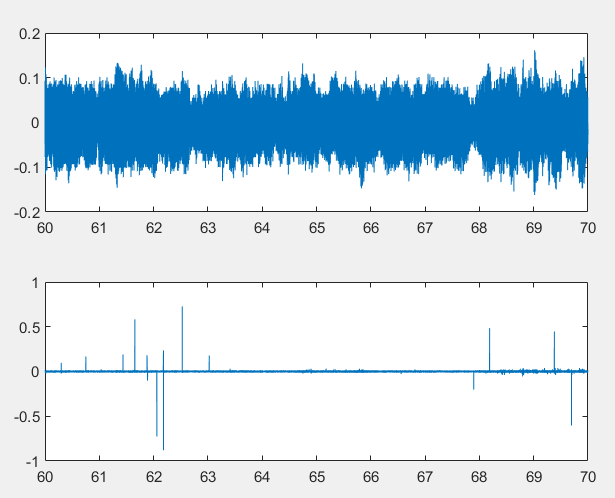
\includegraphics[width=1\textwidth]{images/signalcraquement.png}
    \caption{Zoom sur l'un des craquements.}
    \label{fig-binaire}
\end{figure}


Ecouter le signal restauré. Commentez.\\
\newline
Sur la figure 7, nous pouvons observer que les nombreux pics d'amplitude supérieur à 0.015 ont disparu. Cela indique que notre traitement a fonctionné. Cependant, sur l'erreur quadratique nous pouvons constater que des erreurs persistent. A l'aide de la fonction \textit{sound}, nous avons écouté le morceau modifié mais il semble étouffé. 
\clearpage

\subsection{Restauration par prédiction {\em causale / anticausale}}

La prédiction causale (estimation de l'échantillon $s[n]$ à partir des échantillons antérieurs) de la question \ref{sec:predlin} produit une erreur de prédiction où chaque craquement est repéré par un pic principal, suivi d'un train de pics secondaires (rebonds dus au temps de réponse du filtre $h[k]$). Le débruitage par seuillage de cette erreur de prédiction peut alors conduire à la détection de faux craquements\ldots
Pour éviter cela, on peut procéder à une prédiction causale, combinée à une prédiction anticausale où chaque échantillon 
$s[n]$ est prédit à partir des $M$ échantillons suivants $(s[n+k],\,k=1,\ldots,M)$ et ce, en utilisant le même filtre $h[k]$ puisque la fonction d'autocorrélation est paire. Les erreurs de prédiction $\varepsilon_{\rm causale}$ et $\varepsilon_{\rm anticausale}$ n'ont alors en commun que les pics principaux localisés aux instants des craquements. Il suffit ensuite de remplacer l'échantillon $s[n_{\rm crack}]$ par la moyenne des deux prédictions $\widehat{s}_{\rm causal}[n_{\rm crack}]$ et $\widehat{s}_{\rm anticausal}[n_{\rm crack}]$. \\

Programmez cette solution en expliquant bien chaque étape de la procédure. 
\begin{verbatim}
    % Initialisation des variables 
    p = 1;
    s_chapeau_anticausal = zeros(1,length(s2));
    s_restaur = s2;
    
    % Calcul de la somme anti-causal  
    for n = indice_temps_60:indice_temps_70-20
        somme_anticausal = 0;*
        % Application de la formule : somme de 1 à M de h[k]*S(n+k)
        for k = 1:M
            %s_chapeau_anticausal vaut la somme des s(n+k)
            somme_anticausal = somme_anticausal + h(k)*s(n+k);
        end
        % Ajout de la somme au vecteur anti-causal
        s_chapeau_anticausal(p) = somme_anticausal;
        p = p+1;
    end
    
    % Calcul de l'erreur quadratique anti-causal
    erreur_quad_anticausal = s_chapeau_anticausal-s2';
    
    % Parcours des deux listes pour trouver les indices des craquements 
    inter = intersect(crak,crak_antic);
    
    % Parcours du signal et au besoin, on reconstruie à l'aide de S causal et anti_causal 
    for k = 1:length(inter)
        s_restaur(inter(k)) = (s_chapeau(inter(k)) + s_chapeau_anticausal(inter(k)))/2;
    end
    
    % Partie affichage ---
\end{verbatim}

Affichez le résultat de la restauration ainsi obtenue.

\begin{figure}[!h]
    \centering
    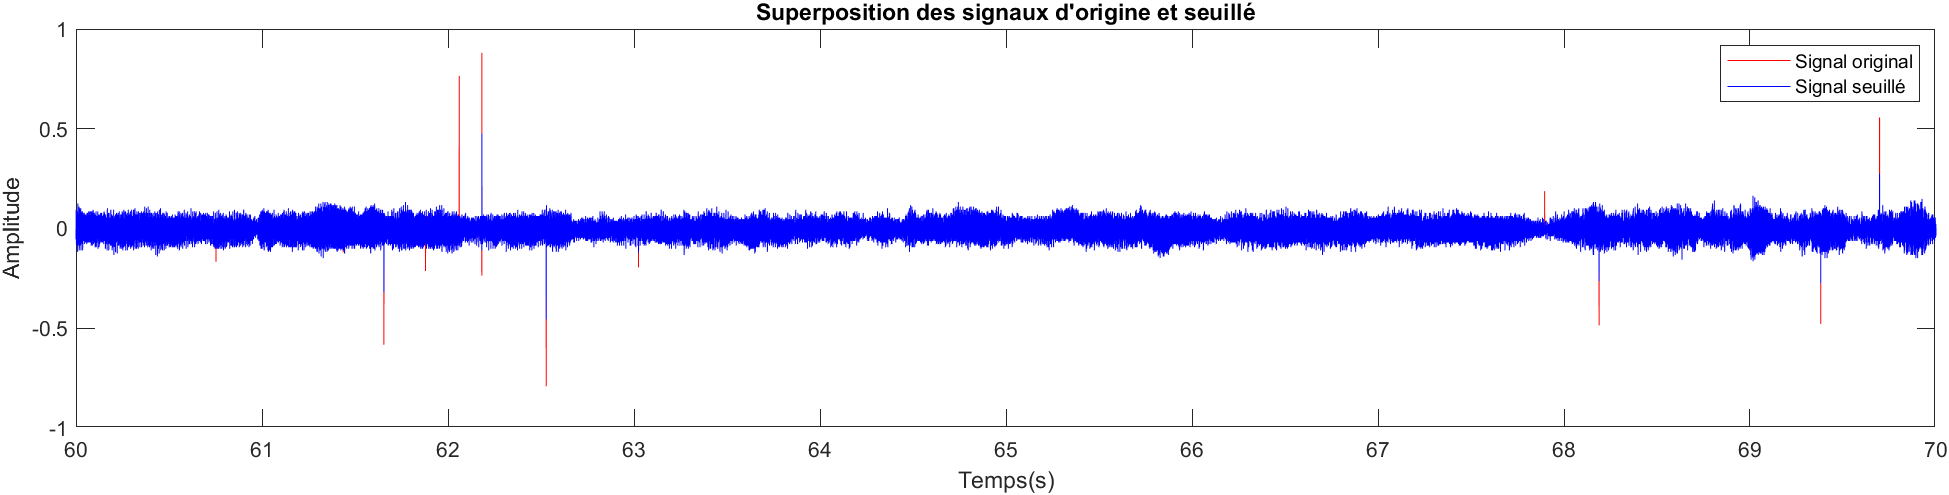
\includegraphics[width=1\textwidth]{images/partie6_signal.png}
    \caption{Signal reconstitué}
    \label{fig-binaire}
\end{figure}
\newpage
\begin{figure}[!h]
    \centering
    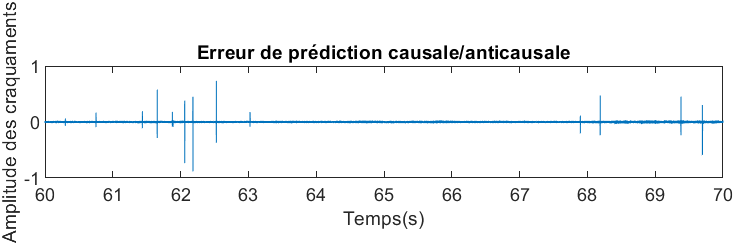
\includegraphics[width=0.7\textwidth]{images/figure2.6.2.png}
    \caption{Erreur quadratique}
    \label{fig-binaire}
\end{figure}

Ecoutez le signal restauré. Concluez.

Pour cette dernière partie, notre méthodologie peut être décomposée en 5 étapes. 1ère partie, nous avons calculé la fonction anti-causale pour $M=20$, ensuite nous calculons la nouvelle erreur quadratique. Dans un troisième temps, nous utilisons le même procédé qu'avec le signal causal pour récupérer les craquement.\\ 
La dernière étape du processus est de comparer les deux vecteurs d'indices, les éléments communs correspondent au craquements. 
Pour finir, on modifie ces éléments en remplaçant dans le signal par la moyenne des deux signaux estimés.\\

Nous avons écouté le signal, et nous constatons qu'il y a une améliorations de qualité car les craquements sont plus discrets sans que cela ait altéré la qualité de la musique.
\end{document}









































